% Use only LaTeX2e, calling the article.cls class and 12-point type.

\documentclass[11pt]{article}
\usepackage[round,semicolon]{natbib}
\usepackage[margin=1.4in]{geometry}
\usepackage{kpfonts}

\usepackage{seqsplit}
\usepackage{placeins}

\usepackage{newfloat}
\usepackage[labelfont=bf]{caption}
\usepackage{nameref}
\usepackage{rotating}
\usepackage{color}
\usepackage{float}

\setcounter{topnumber}{8}
\setcounter{bottomnumber}{8}
\setcounter{totalnumber}{8}

\usepackage{newfloat}
\DeclareFloatingEnvironment[name={Figure}]{suppfigure}
\renewcommand{\thesuppfigure}{S\arabic{suppfigure}}

\definecolor{darkblue}{rgb}{0, 0.0, 0.6}

\usepackage{hyperref}
\hypersetup{colorlinks,citecolor=blue,linkcolor=darkblue,urlcolor=blue}

\usepackage{seqsplit}

\usepackage{array}
\newcolumntype{R}[1]{>{\raggedright\arraybackslash}p{#1}}
\newcolumntype{C}[1]{>{\centering\let\newline\\\arraybackslash\hspace{0pt}}m{#1}}

\newcommand{\comment}[1]{{\color{red}[\textsl{#1}]}}

\usepackage{setspace}

\renewcommand{\topfraction}{1}
\renewcommand{\bottomfraction}{1}
\renewcommand{\textfraction}{0}
\renewcommand{\floatpagefraction}{1}

%\renewcommand{\abstractname}{\large SUMMARY}


\title{Quantifying the ease of viral escape from broad and narrow antibodies to influenza hemagglutinin} 

\author
{Michael B. Doud$^{1,2,3,\dagger}$, Juhye M. Lee$^{1,2,3,\dagger}$, and Jesse D. Bloom$^{1,2,*}$\\
\\
\scriptsize{$^1$Basic Sciences and Computational Biology Program, Fred Hutchinson Cancer Research Center}\\
\scriptsize{$^2$Department of Genome Sciences and $^3$Medical Scientist Training Program, University of Washington} \\
\scriptsize{Seattle, WA, USA} \\
\scriptsize{$^{\dagger}$These authors contributed equally} \\
\scriptsize{$^*$Correspondence: \href{jbloom@fredhutch.org}{jbloom@fredhutch.org}}
}

\date{}


\begin{document}

\maketitle
\onehalfspacing

\begin{abstract}
Influenza virus can completely escape most antibodies with single mutations.
However, rare antibodies broadly neutralize many viral strains.
It is unclear how easily influenza virus might escape such broad antibodies if they became widespread due to therapeutic use or vaccination.
Here we map all single amino-acid mutations that increase resistance to broad antibodies targeting hemagglutinin.
Crucially, our approach not only identifies antigenic mutations but also quantifies their effect sizes.
All antibodies select mutations, but the effect sizes vary widely. 
The virus can escape a broad antibody targeting hemagglutinin's receptor-binding pocket the same way it escapes narrow strain-specific antibodies: via single mutations with huge effects.   
In contrast, broad antibodies targeting hemagglutinin's stalk only select mutations with small antigenic effects. 
Therefore, antibody breadth is not necessarily an indicator of the difficulty of viral escape.
Broad antibodies targeting hemagglutinin's stalk are quantifiably harder to escape than antibodies targeting hemagglutinin's head or receptor-binding pocket.
\end{abstract}

\section*{INTRODUCTION}
Nearly all viruses show some antigenic variation.
However, the extent of this variation ranges widely.
For instance, although both measles virus~\citep{birrer1981antigenic,ter1981antigenic} and polio virus~\citep{crainic1983natural,diamond1985antigenic,drexler2014robustness} exhibit antigenic variation, the magnitude of this variation is small. 
Therefore, immunity to both these viruses is lifelong~\citep{?}.
In contrast, human influenza virus exhibits extensive antigenic variation.
So although infection with an influenza virus strain provides lifelong immunity to that exact strain~\citep{?}, the virus's rapid antigenic evolution erodes the effectiveness of this immunity to that strain's descendents within just a few years~\citep{?}.

One possible reason that different viruses exhibit different amounts of antigenic variation is that they may have disparate evolutionary capacities to escape the antibodies that are immunodominant during natural immune responses~\citep{lipsitch2007patterns,cobey2014pathogen,fulton2015mutational}.
According to this explanation, human influenza virus undergoes rapid antigenic drift because most neutralizing antibodies target epitopes on the viral hemagglutinin protein that are highly tolerant of mutational change.
This explanation is supported by classic experiments showing that it is easy to select viral mutants that escape most antibodies~\citep{yewdell1979antigenic,webster1980determination}, as well as by the observation that mutations that alter antigenicity arise frequently during influenza's evolution globally~\citep{koel2013substitutions,chambers2015identification,petrie2016antibodies,neher2016prediction} and within individual humans with long-term infections~\citep{xue2017parallel}.
A corollary of this explanation is that the virus's capacity for antigenic drift would be reduced if most antibodies instead targeted epitopes that were less mutationally tolerant.

Verifying this corollary has become of practical importance with the discovery of broadly neutralizing antibodies against influenza virus.
These antibodies typically target conserved epitopes in hemagglutinin's stalk~\citep{?} or receptor-binding pocket~\citep{?}, and neutralize a wide range of viral strains.
Broad antibodies usually make only a modest contribution to natural human immunity, since they are less abundant than antibodies to antigenically variable epitopes on the head of hemagglutinin~\citep{?}.
However, major efforts are underway to elicit broad antibodies by vaccination~\citep{?} or administer them directly as therapeutics or prophylactics~\citep{?}.

If these efforts succeed, the epitopes of broad antibodies will be under strong antigenic selection in human influenza virus.
Would such selection then drive extensive antigenic variation in these epitopes?
There is precedent for the idea that the immune status of the host population can shape influenza virus antigenic evolution: the virus undergoes faster antigenic drift in long-lived humans that accumulate immune memory than in short-lived swine that are mostly naive~\citep{sheerar1989antigenic,luoh1992hemagglutinin}, and poultry vaccination may accelerate antigenic drift of avian influenza~\citep{lee2004effect}.
But alternatively, perhaps broad antibodies are broad because the virus has difficulty escaping from them regardless of the selection from host immunity.

So far, there is limited data addressing whether the epitopes of broad antibodies are inherently resistant to viral antigenic evolution.
Several studies have shown that the globular head domain of hemagglutinin is less mutationally tolerant than the stalk domain where many broad antibodies bind~\citep{thyagarajan2014inherent,wu2014high,heaton2013genome}.
However, these studies did not select for actual antibody escape, so it is difficult to directly relate their measurements to the virus's evolutionary capacity under immune selection.
Other work has selected antigenic mutants with a few broad antibodies~\citep{?}, demonstrating that these epitopes are not entirely refractory to change.
But given that antibodies can select some antigenic variation even in measles virus~\citep{?} and polio virus~\citep{?}, the existence of mutations selectable by broad antibodies does not necessarily imply that influenza virus can escape these antibodies with ease.
The fundamental problem is that none of these studies provide quantitative data on the ease of viral escape that can be compared across antibodies in an apples-to-apples fashion.

Here we systematically quantify the ease with which influenza virus can escape from a range of broad and narrow antibodies via single amino-acid mutations.
Specifically, we impose antibody selection on libraries of viruses carrying all amino-acid mutants of hemagglutinin compatible with viral replication, and then measure the fraction of virions with each mutation that survive the selection at several antibody concentrations.
Critically, this approach quantifies the \emph{magnitude} of the antigenic effect of every mutation in a way that can be directly compared across antibodies.
We find that even the broadest antibodies can select mutations that increase the virus's resistance to neutralization.
However, the magnitudes of the antigenic effects vary greatly across antibodies.
Single mutations can make the virus completely resistant to both narrow strain-specific antibodies and a broad antibody against the receptor-binding pocket.
But no single mutation does more than modestly increase the virus's resistance to broad antibodies against the hemagglutinin stalk.
These results suggest that systematically quantifying the antigenic effects of all single amino-acid mutations is a useful complement to simply measuring antibody breadth when trying to assess the potential for antigenic drift. 


%Broadly neutralizing antibodies against influenza virus are of great interest... \cite{corti2017tackling}. 




\section*{RESULTS}

\subsection*{A method to quantify the ease of escape.}
\comment{Jesse writes a draft of this section.}
\begin{figure}
\centerline{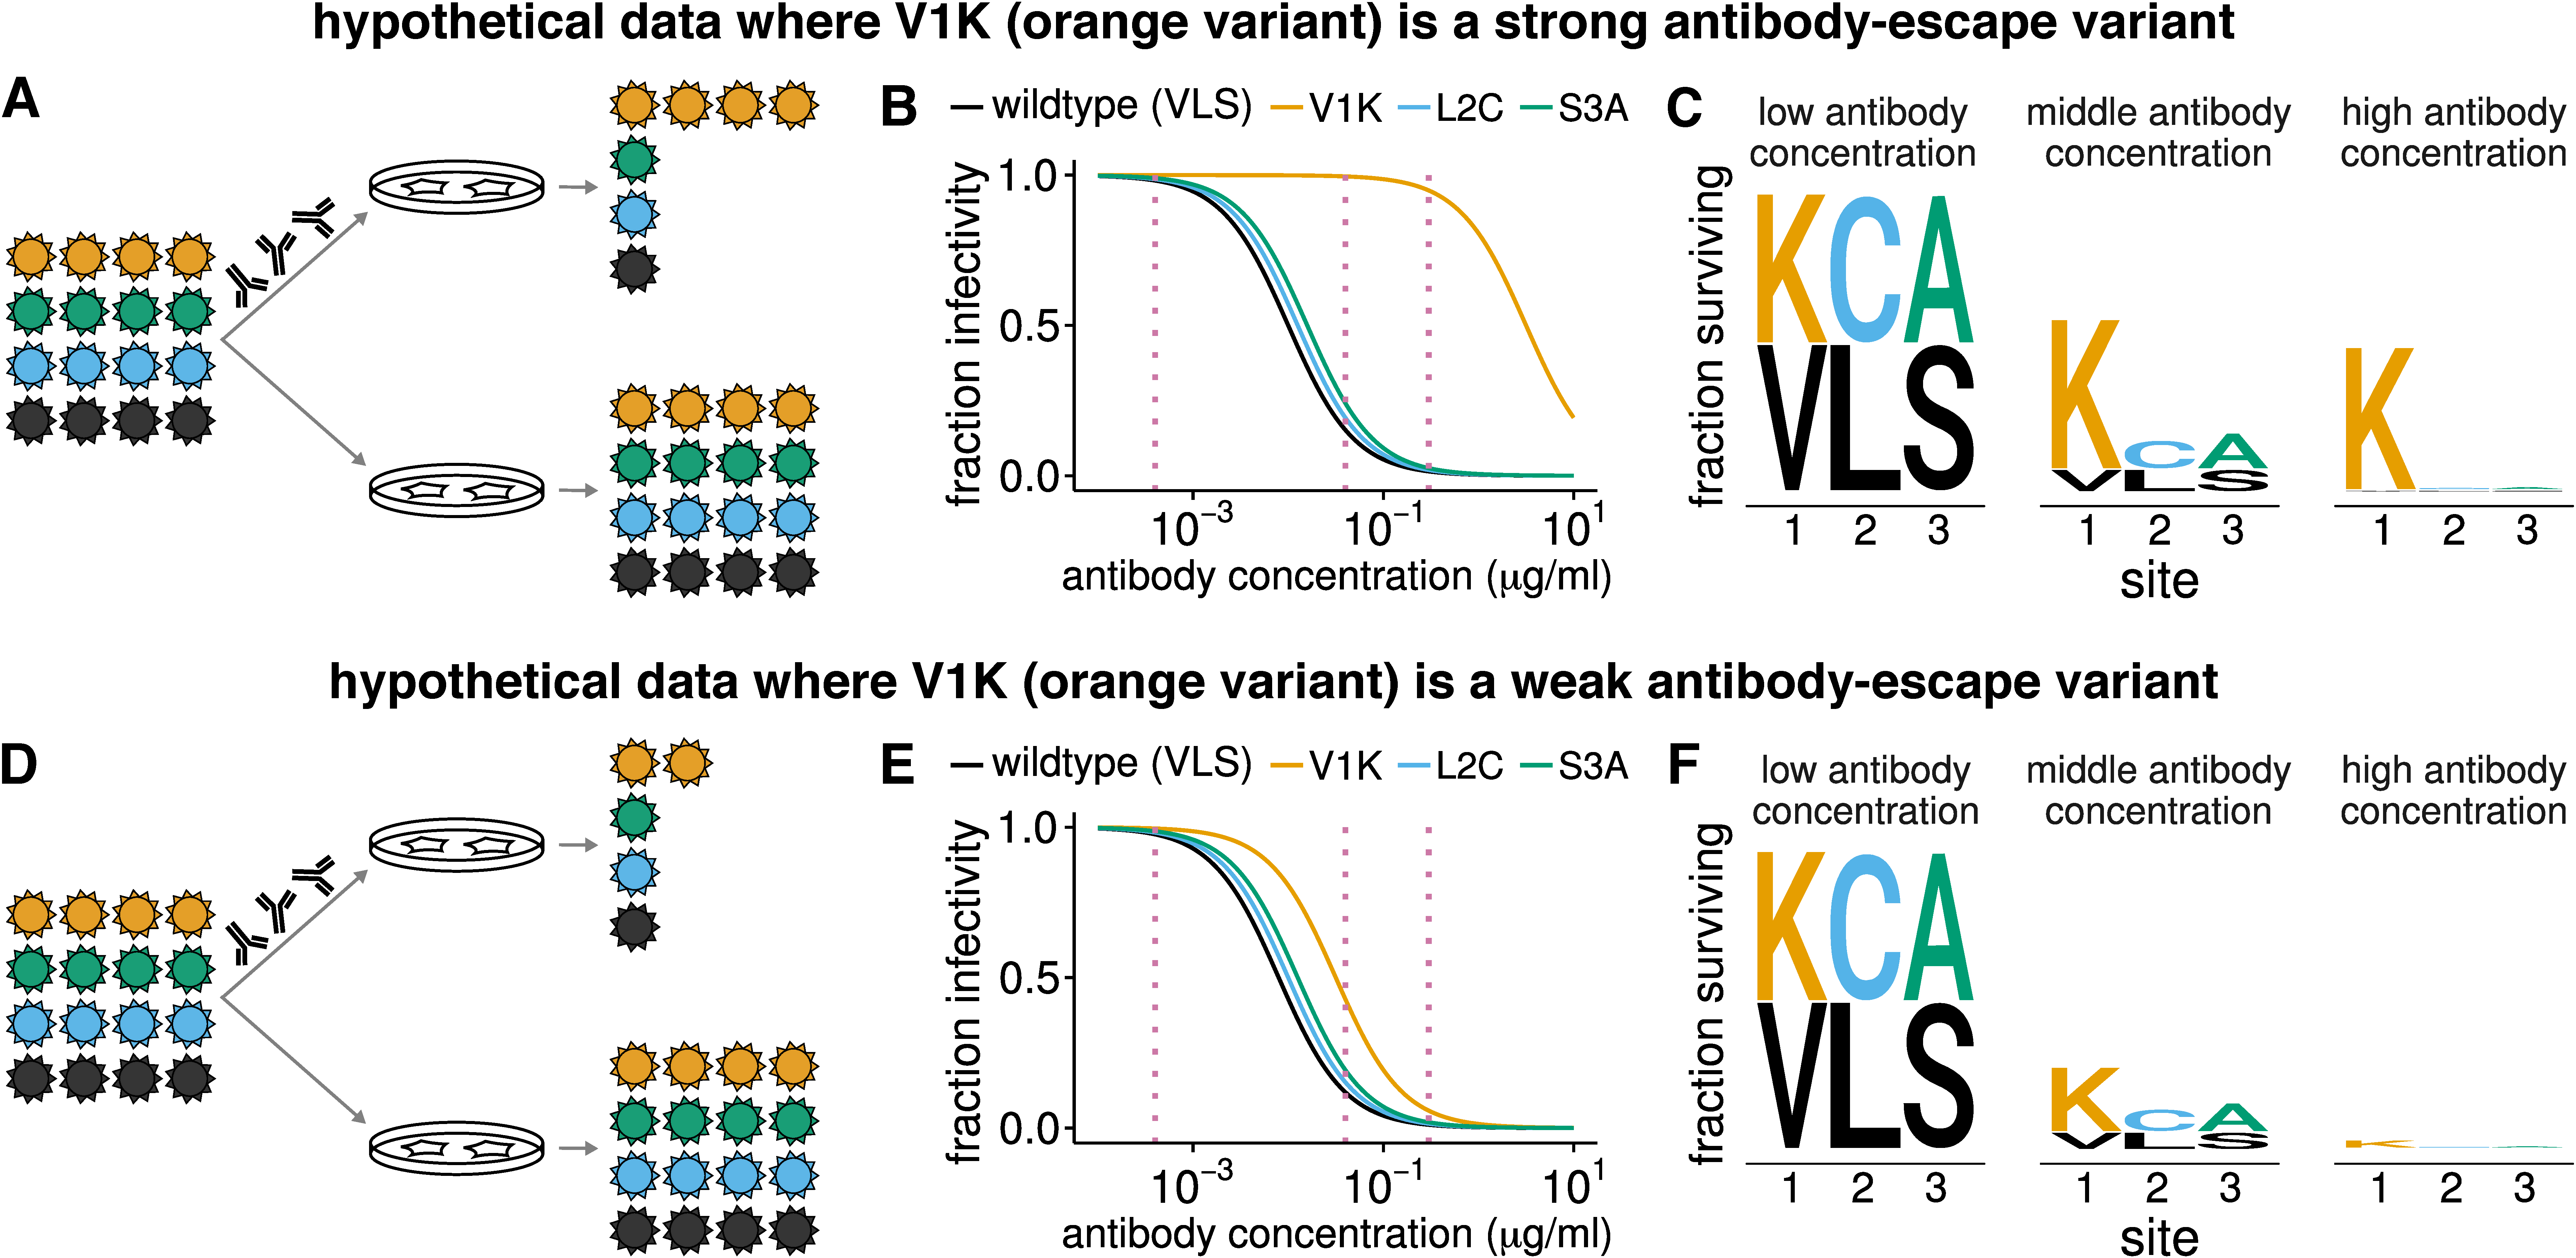
\includegraphics[width=\textwidth]{figs/fracsurvive_example/fracsurvive_fig.pdf}}
\caption{\label{fig:fracsurvive_example}
CAPTION
}
\end{figure}

\subsection*{Broad and narrow antibodies that neutralize influenza virus hemagglutinin}
\comment{Juhye writes a draft of this section.}

% blurbs about the specific antibodies we use here:
C179 isolation and escape mutant selection \cite{okuno1993common}.
C179 structure with 1957 H2, binding data to many strains, and citations to older studies demonstrating C179 cross-neutralization to H1, H2, H5, H6, and H9:  \cite{dreyfus2013structure}.
FI6v3 was isolated... \cite{corti2011neutralizing}.
S139/1 isolation and selection of escape mutants from Aichi H3, Adachi H2, and WSN H1: \cite{yoshida2009cross}.
S139/1 structure with Victoria75 H3 and binding/neutralization data: \cite{lee2012heterosubtypic}.

\begin{figure}
\centerline{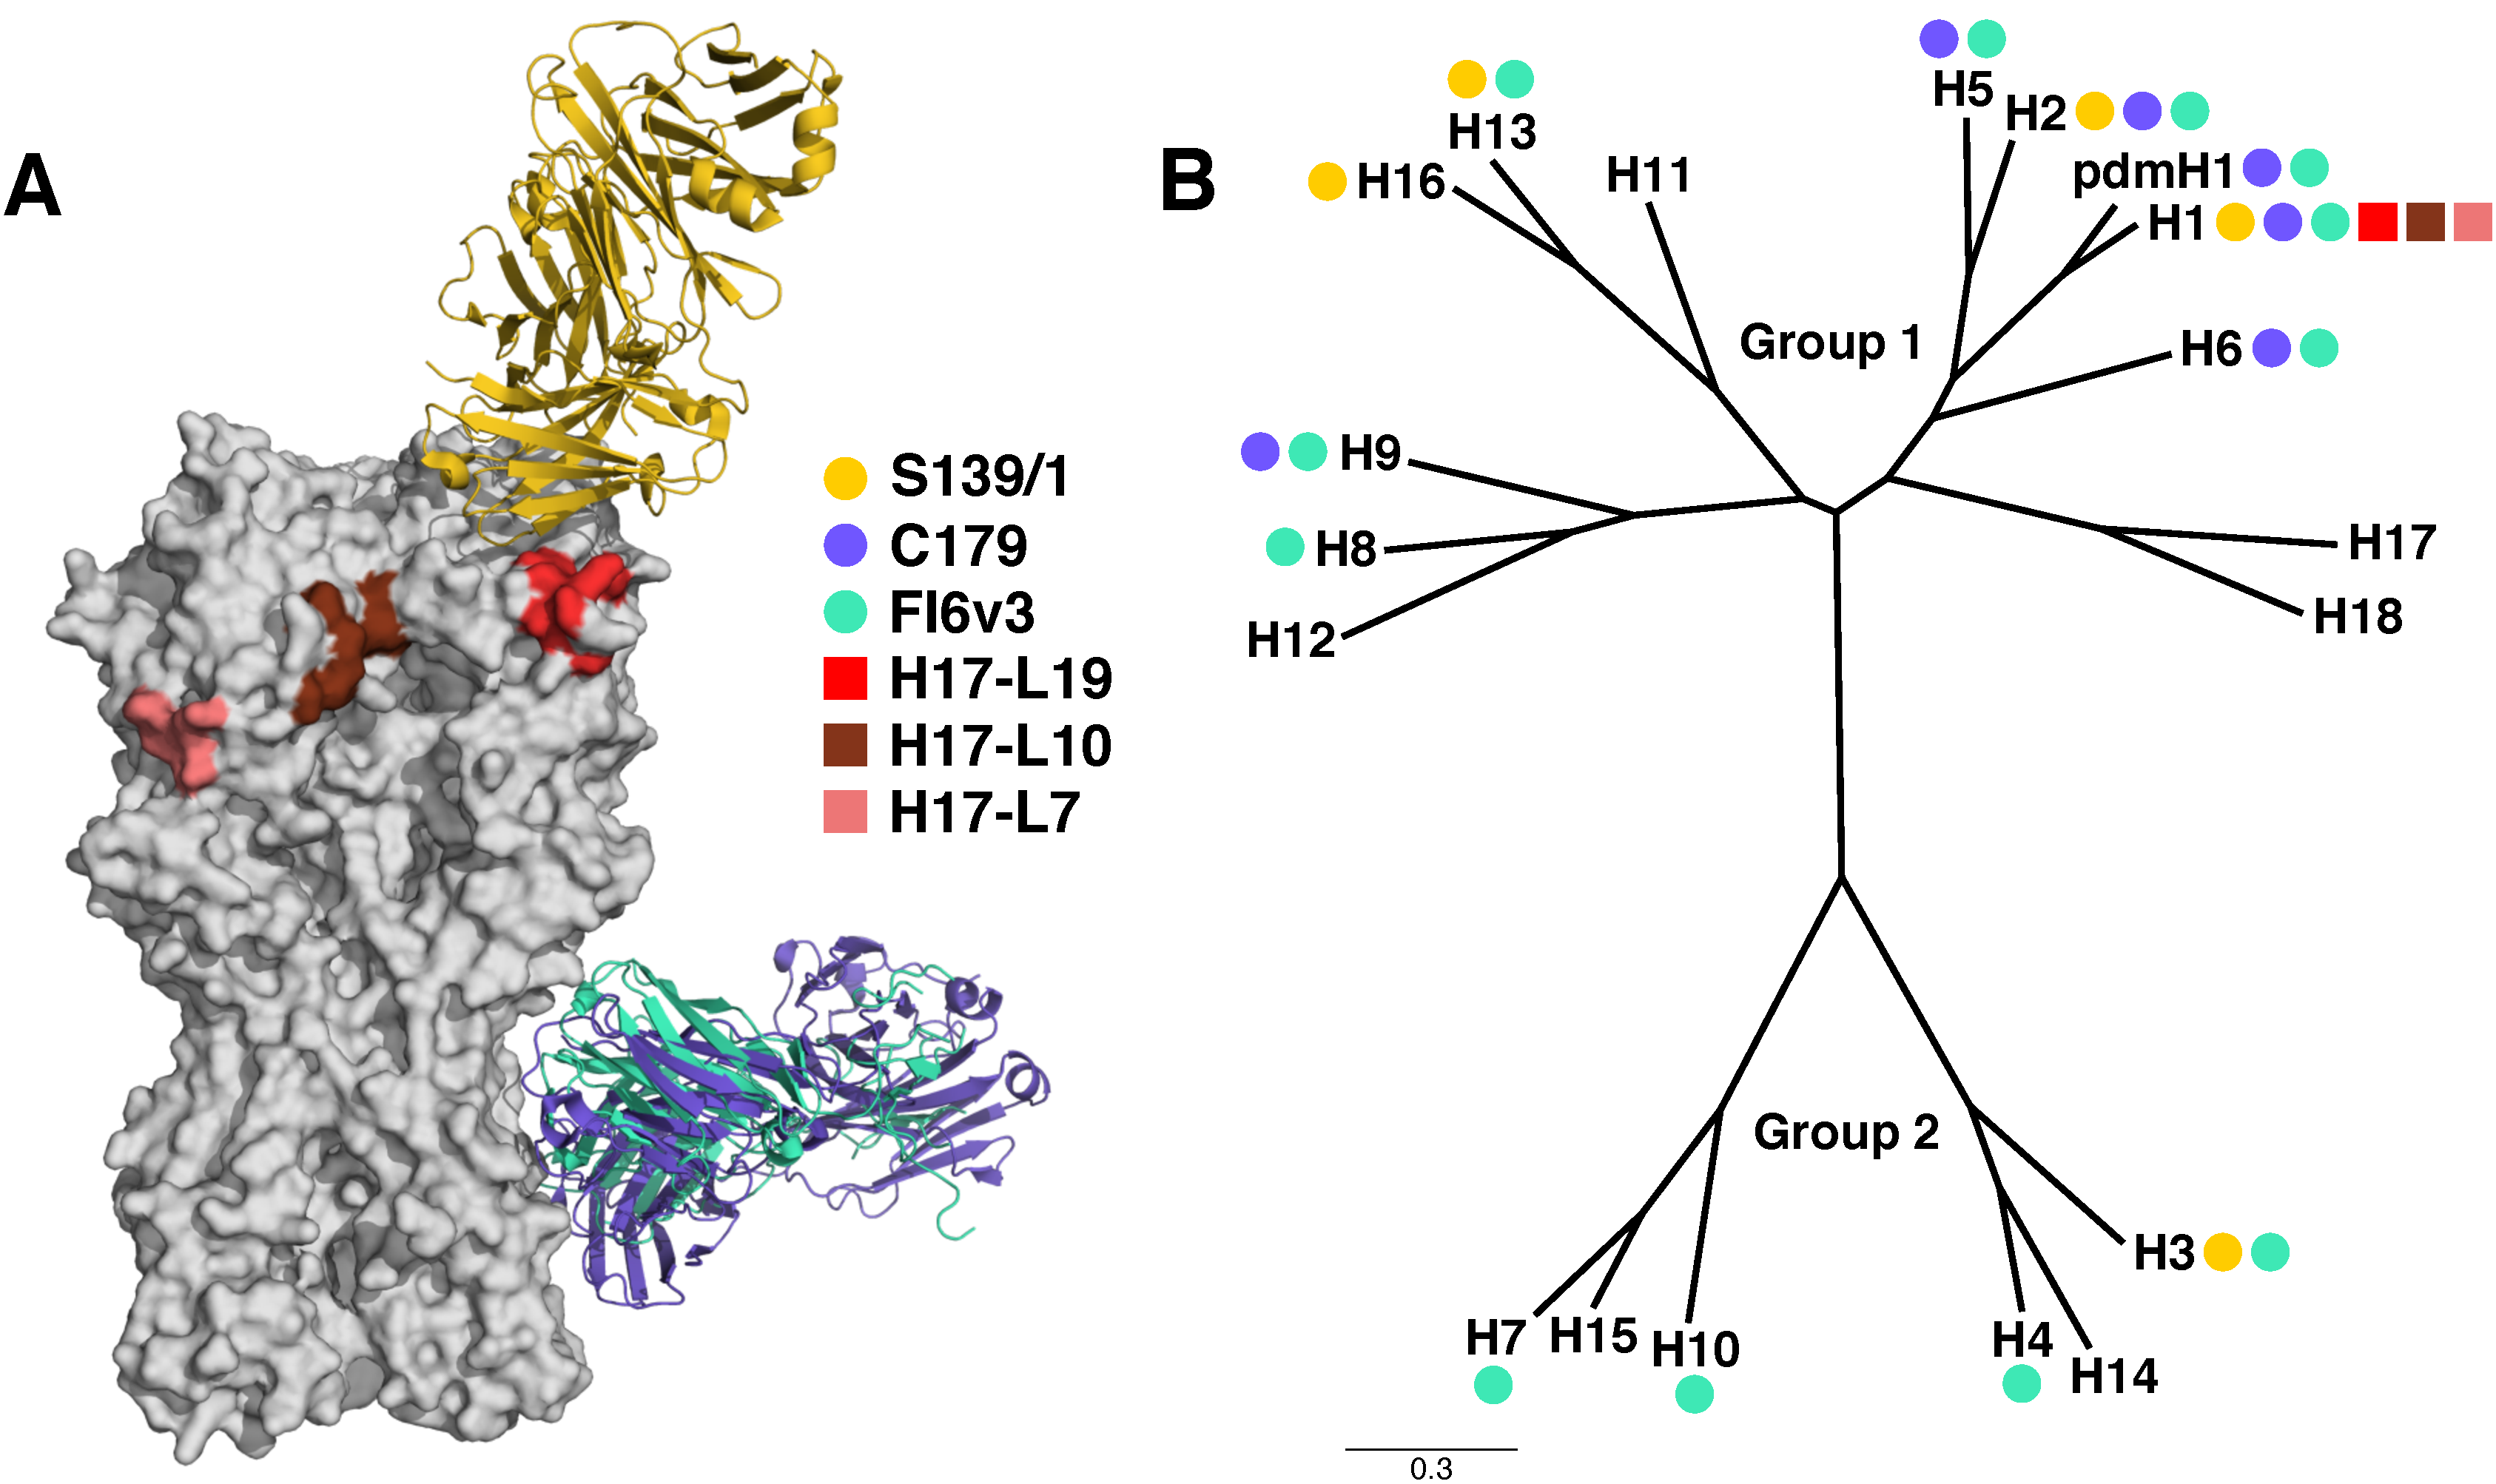
\includegraphics[width=\textwidth]{figs/antibody_summary_fig/Ab_summary.pdf}}
\caption{\label{fig:antibody_summary}
CAPTION
}
\end{figure}


\begin{figure}
\centerline{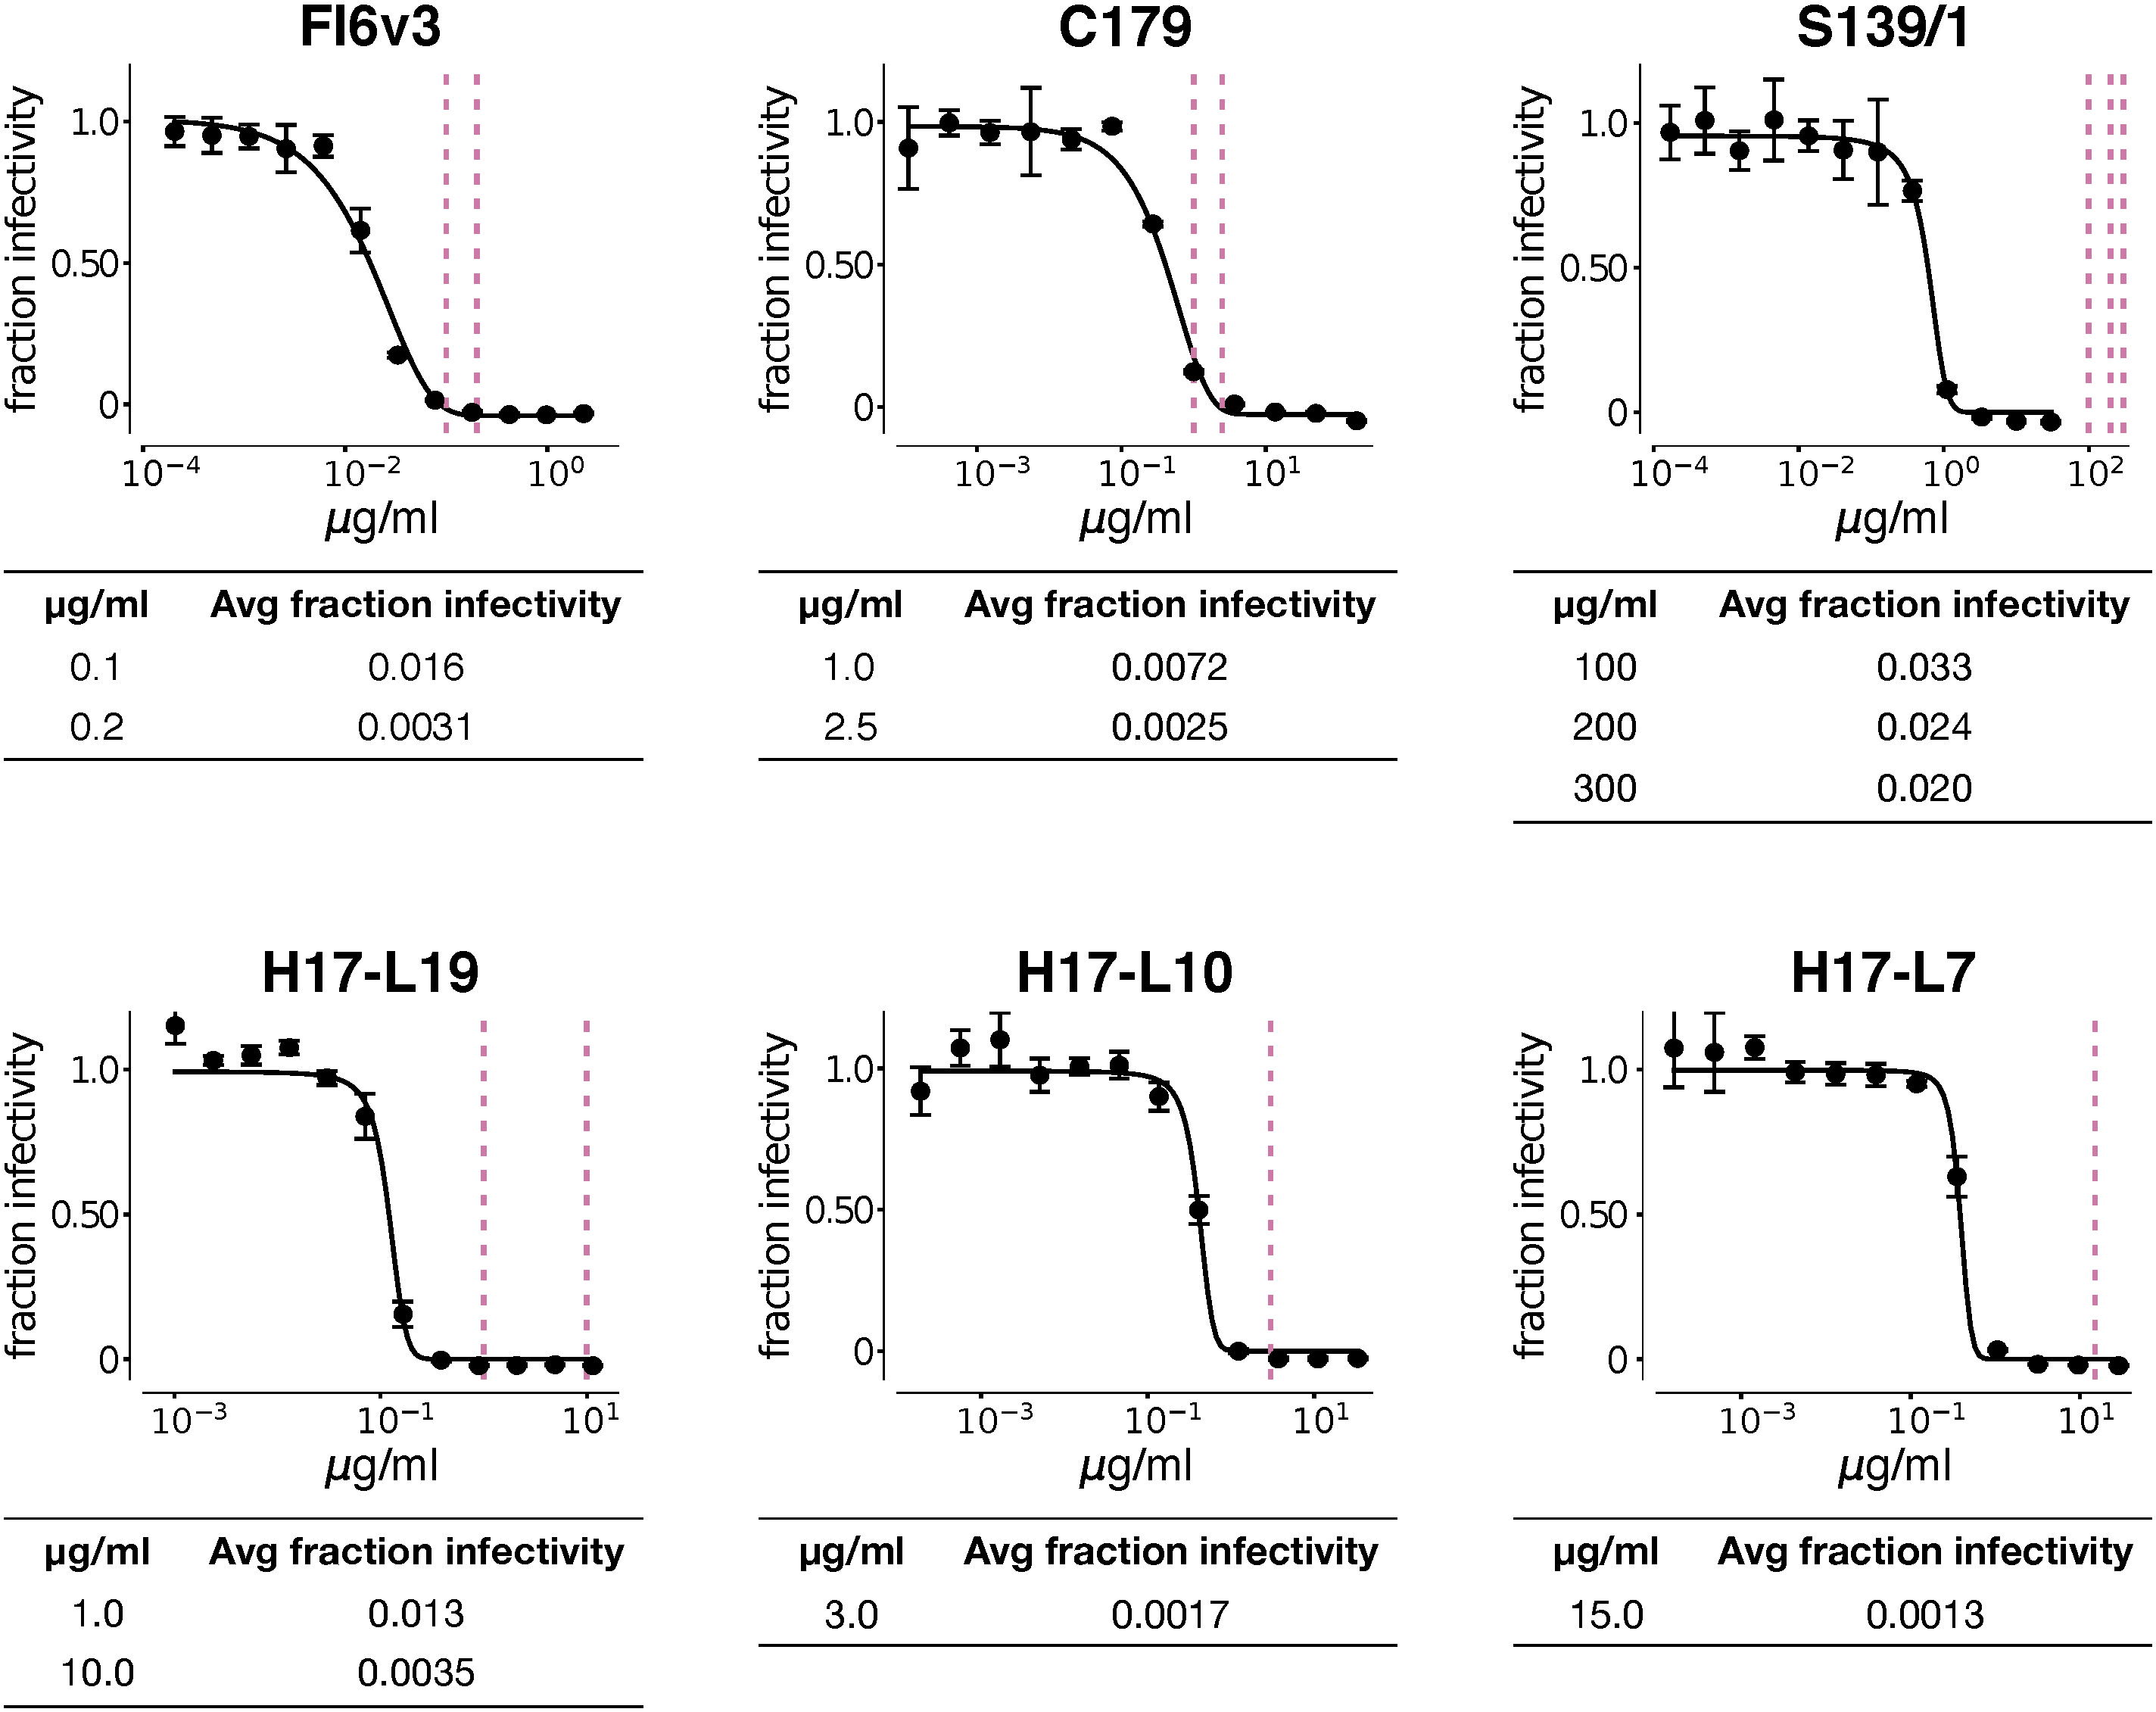
\includegraphics[width=0.8\textwidth]{figs/neutralization_curves/WT_neutralization_curves.pdf}}
\caption{\label{fig:neutcurves}
CAPTION
\comment{
Get rid of the panel numbers altogether and just have the antibody names.
}
}
\end{figure}

\subsection*{Ease of escape from each antibody}
\comment{Jesse can work on a rough draft of this section.}

\comment{Juhye, can you create a correlation among replicates supplemental figure. In the \texttt{./figs/corrs/} directory are all the plots. Is it possible to nicely arrange them on one page, maybe getting rid of the diagonals?}

\begin{figure}
\centerline{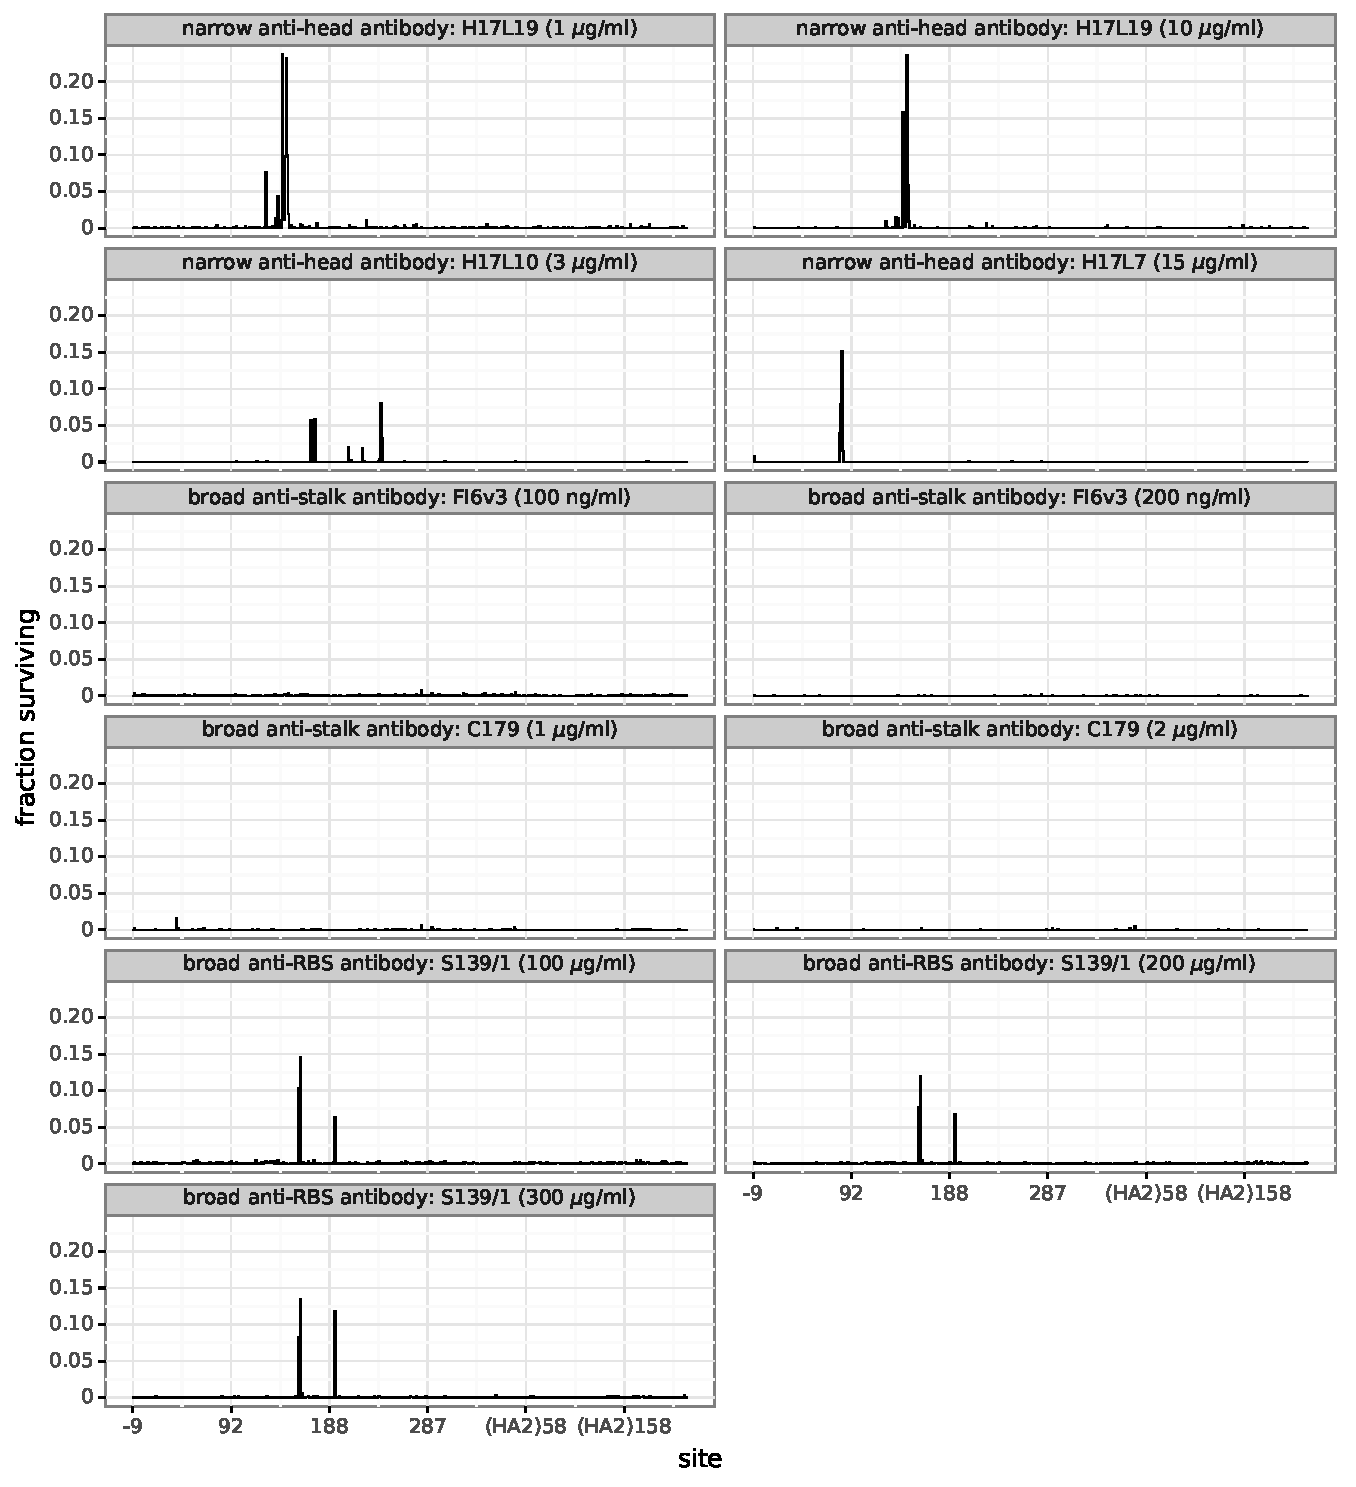
\includegraphics[width=\textwidth]{figs/avgfracsurvive.pdf}}
\caption{
\label{fig:avgfracsurvive}
CAPTION
Figure~\ref{suppfig:maxfracsurvive} shows the fraction surviving for the single most strongly selected amino-acid mutation at each site.
}
\end{figure}

\subsection*{For all antibodies, the selected sites of escape occur in the antibody binding footprints}

\section*{DISCUSSION}
Some discussion

\clearpage

\section*{METHODS}
\subsection*{Antibodies}
FI6v3 was expressed and purified by the Fred Hutchinson Cancer Research Center protein expression core \comment{i think?}.
C179 was purchased from Takara Bio Inc (Catalog \# M145).
S139/1 heavy and light chain variable sequences were obtained from PDB ID 4GMS~\cite{lee2012heterosubtypic} and expressed and purified by the Fred Hutchinson Cancer Research Center protein expression core.

\subsection*{Mutant virus selections with antibody}
Library selections, deep sequencing, and computation of mutation differential selection were performed as previously described~\cite{doud2017complete}. Briefly, ...

\subsection*{Computation of the fraction $\phi_{r,a}$ of each mutation that escapes antibody neutralization}
\comment{depending on how much of paper focus is on this new metric, some of this rationale might be better placed in the results section}

Mutation differential selection values $s_{r,a}$ reflect the enrichment of a mutation in an antibody-selected sample relative to a mock-selected control. 
The extent of these mutation enrichments are dependent on the stringency of the neutralization: as the concentration of an antibody used to neutralize the mutant virus library is increased, a larger proportion of the virus library is neutralized, and escape mutants become more enriched in the antibody-selected sample relative to the control sample~\cite{doud2017complete}.
Consequently, due to differences in the concentrations and potencies of various antibodies used in mutational antigenic profiling, quantitative comparisons of the effects of mutations on neutralization escape between various antibodies is confounded by differences in neutralization stringency across experiments.

We defined a new metric that accounts for the neutralization stringency of each experiment so that quantitative comparisons can be made between experiments with varying neutralization stringencies.
This new measure, $\phi_{r,a}$, is roughly analogous to the fraction of mutant viruses carrying mutation $a$ at site $r$ that escape neutralization by a given antibody.
The computation of $\phi_{r,a}$ incorporates information about the stringency of neutralization. 
We define this as  $\gamma$ = (100 - \% neutralization)/100), the fraction of library remaining infectious after antibody neutralization measured by qRT-PCR for each antibody-selection experiment as previously described~\cite{doud2017complete}.

Define $\hat{n}_{r,a}^{sel}$ and $\hat{n}_{r,a}^{mock}$ as the number of error-corrected counts of amino-acid mutant $a$ at site $r$ as defined in~\cite{doud2017complete}, and $N_r^{sel}$ and $N_r^{mock}$ be the total counts at site $r$, as specified for either an antibody selection or matched mock condition.
Let $P$ be a pseudocount (default to 5 in these analyses) added to amino-acid counts, and let $f_{r}^{sel}$ and $f_{r}^{mock}$ be relative depths of the selected and mock samples at site $r$ for the purposes of scaling the pseudocount by relative read depth as previously described~\cite{doud2017complete}.

Define the pseudocount-adjusted frequency $\rho$ of mutant $a$ at site $r$ in selected and mock samples to be:
$$\rho_{r,a}^{sel} = \frac{n_{r,a}^{sel}+f_r^{sel}\times P}{N_r^{sel}+f_r^{sel}\times  P}$$
$$\rho_{r,a}^{mock} = \frac{n_{r,a}^{mock}+f_r^{mock}\times P}{N_r^{mock}+f_r^{mock}\times  P}$$

We define $\phi_{r,a}$ as the net `fraction' of mutant $a$ at site $r$ escaping neutralization (above the average escape fraction $\gamma$), and compute this as:
$$\phi_{r,a} = \frac{\gamma \times \rho_{r,a}^{sel}}{\rho_{r,a}^{mock}} - \gamma$$

By this definition, mutations with no effect on antibody escape will have $\phi_{r,a} =0$, and mutations completely escaping antibody will have $\phi_{r,a} \approx 1$.
Care should be taken in interpreting the absolute values of $\phi$, however, since the choice of pseudocount affects the range of $\phi$ values (but not, importantly, the relationships of $\phi$ distributions across antibodies).
We have found that a value of $P=5$ pseudocounts results in $\phi$ values that are roughly bounded from 0 to 1, and consistently use $P=5$ all analyses.

\subsection*{Data availability and source code}
Deep sequencing data has been deposited at the Sequence Read Archive under BioSample accession (\comment{should probably deposit all the new data into the existing biosample SAMN05789126 (Sample name: WSN/1933 HA mutant libraries selected by monoclonal antibodies), which is under bioproject PRJNA309339}).




\clearpage

\small
\subsection*{ACKNOWLEDGMENTS}
This work was supported by grants R01GM102198 and R01AI127893 from the NIGMS and NIAID of the NIH.
MBD was supported in part by training grant T32AI083203 from the NIAID of the NIH.
JML was supported in part by \comment{CIDID grant}.
The research of JDB is supported in part by a Faculty Scholar Grant from the Howard Hughes Medical Institute and the Simons Foundation.

\bibliographystyle{mbe}
\bibliography{references.bib}

\clearpage
\normalsize

\section*{Supplementary Material}
\FloatBarrier

\begin{suppfigure}
\centerline{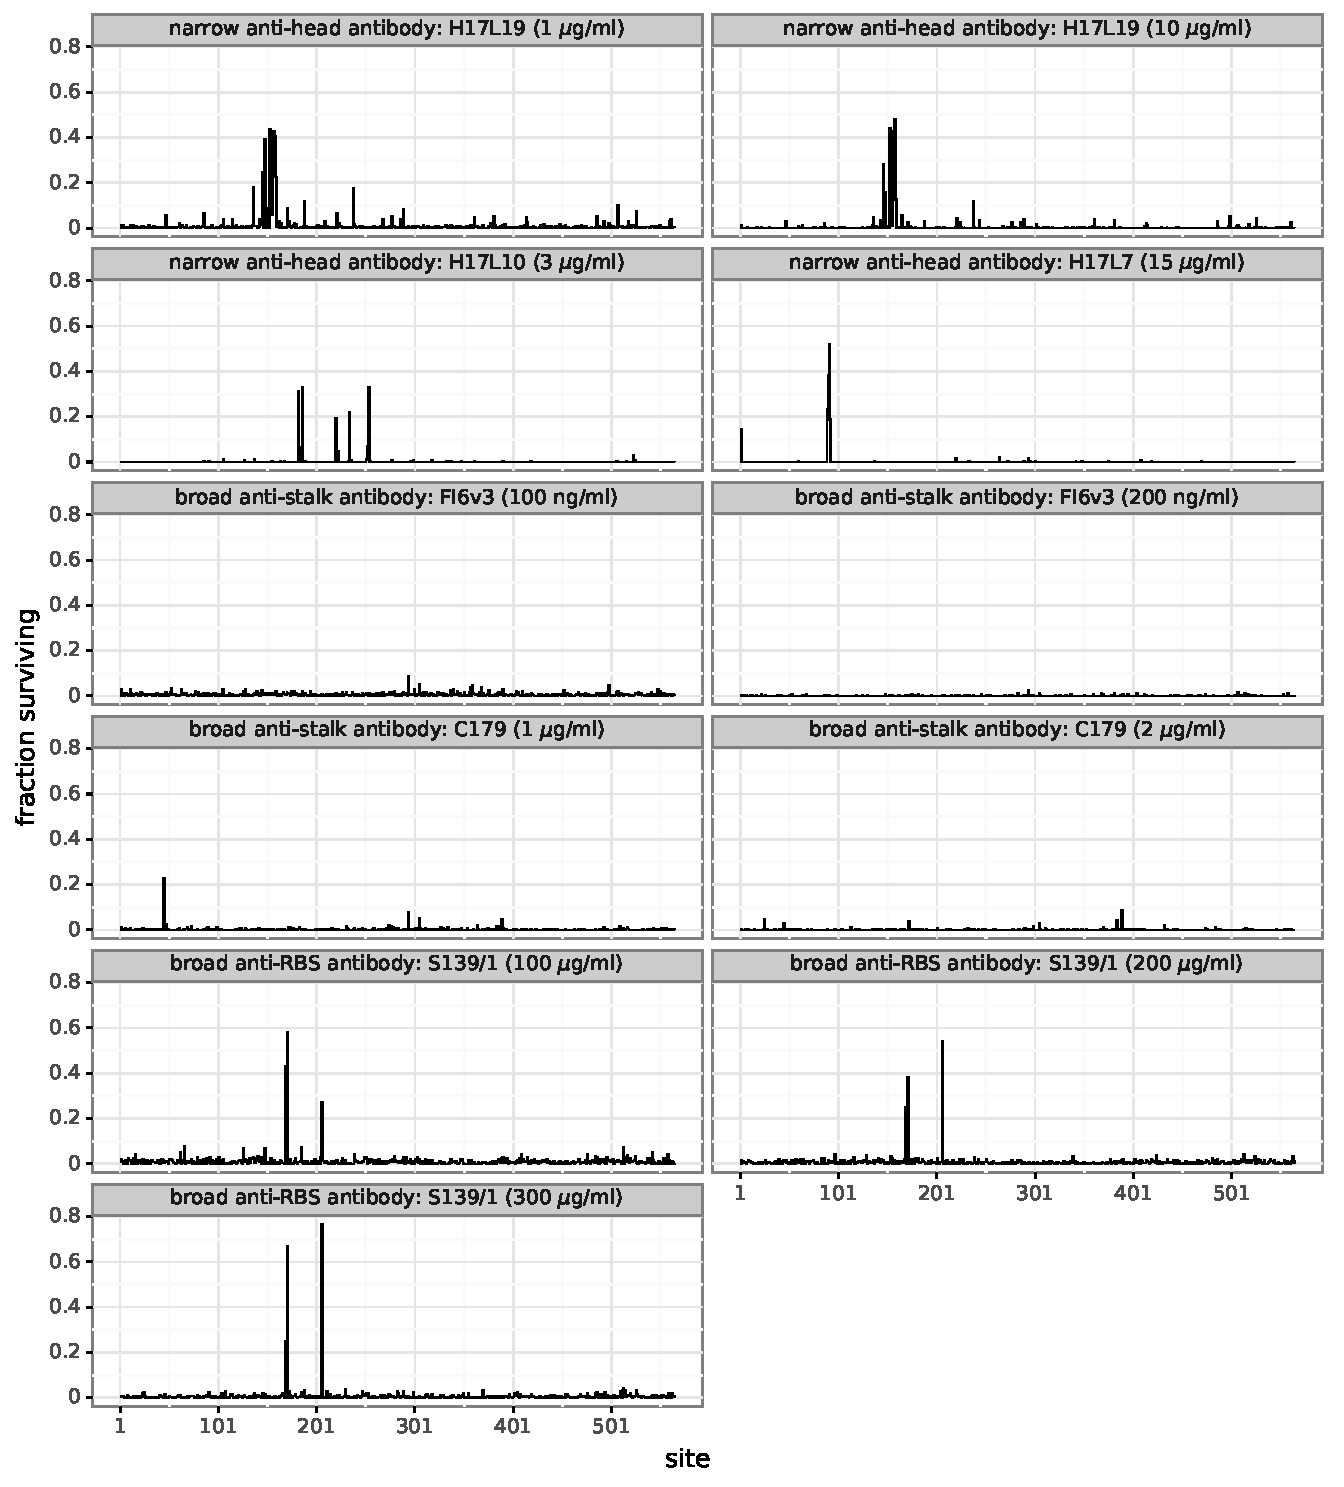
\includegraphics[width=\textwidth]{figs/maxfracsurvive.pdf}}
\caption{\label{suppfig:maxfracsurvive}
CAPTION}
\end{suppfigure}

\begin{suppfigure}
\centerline{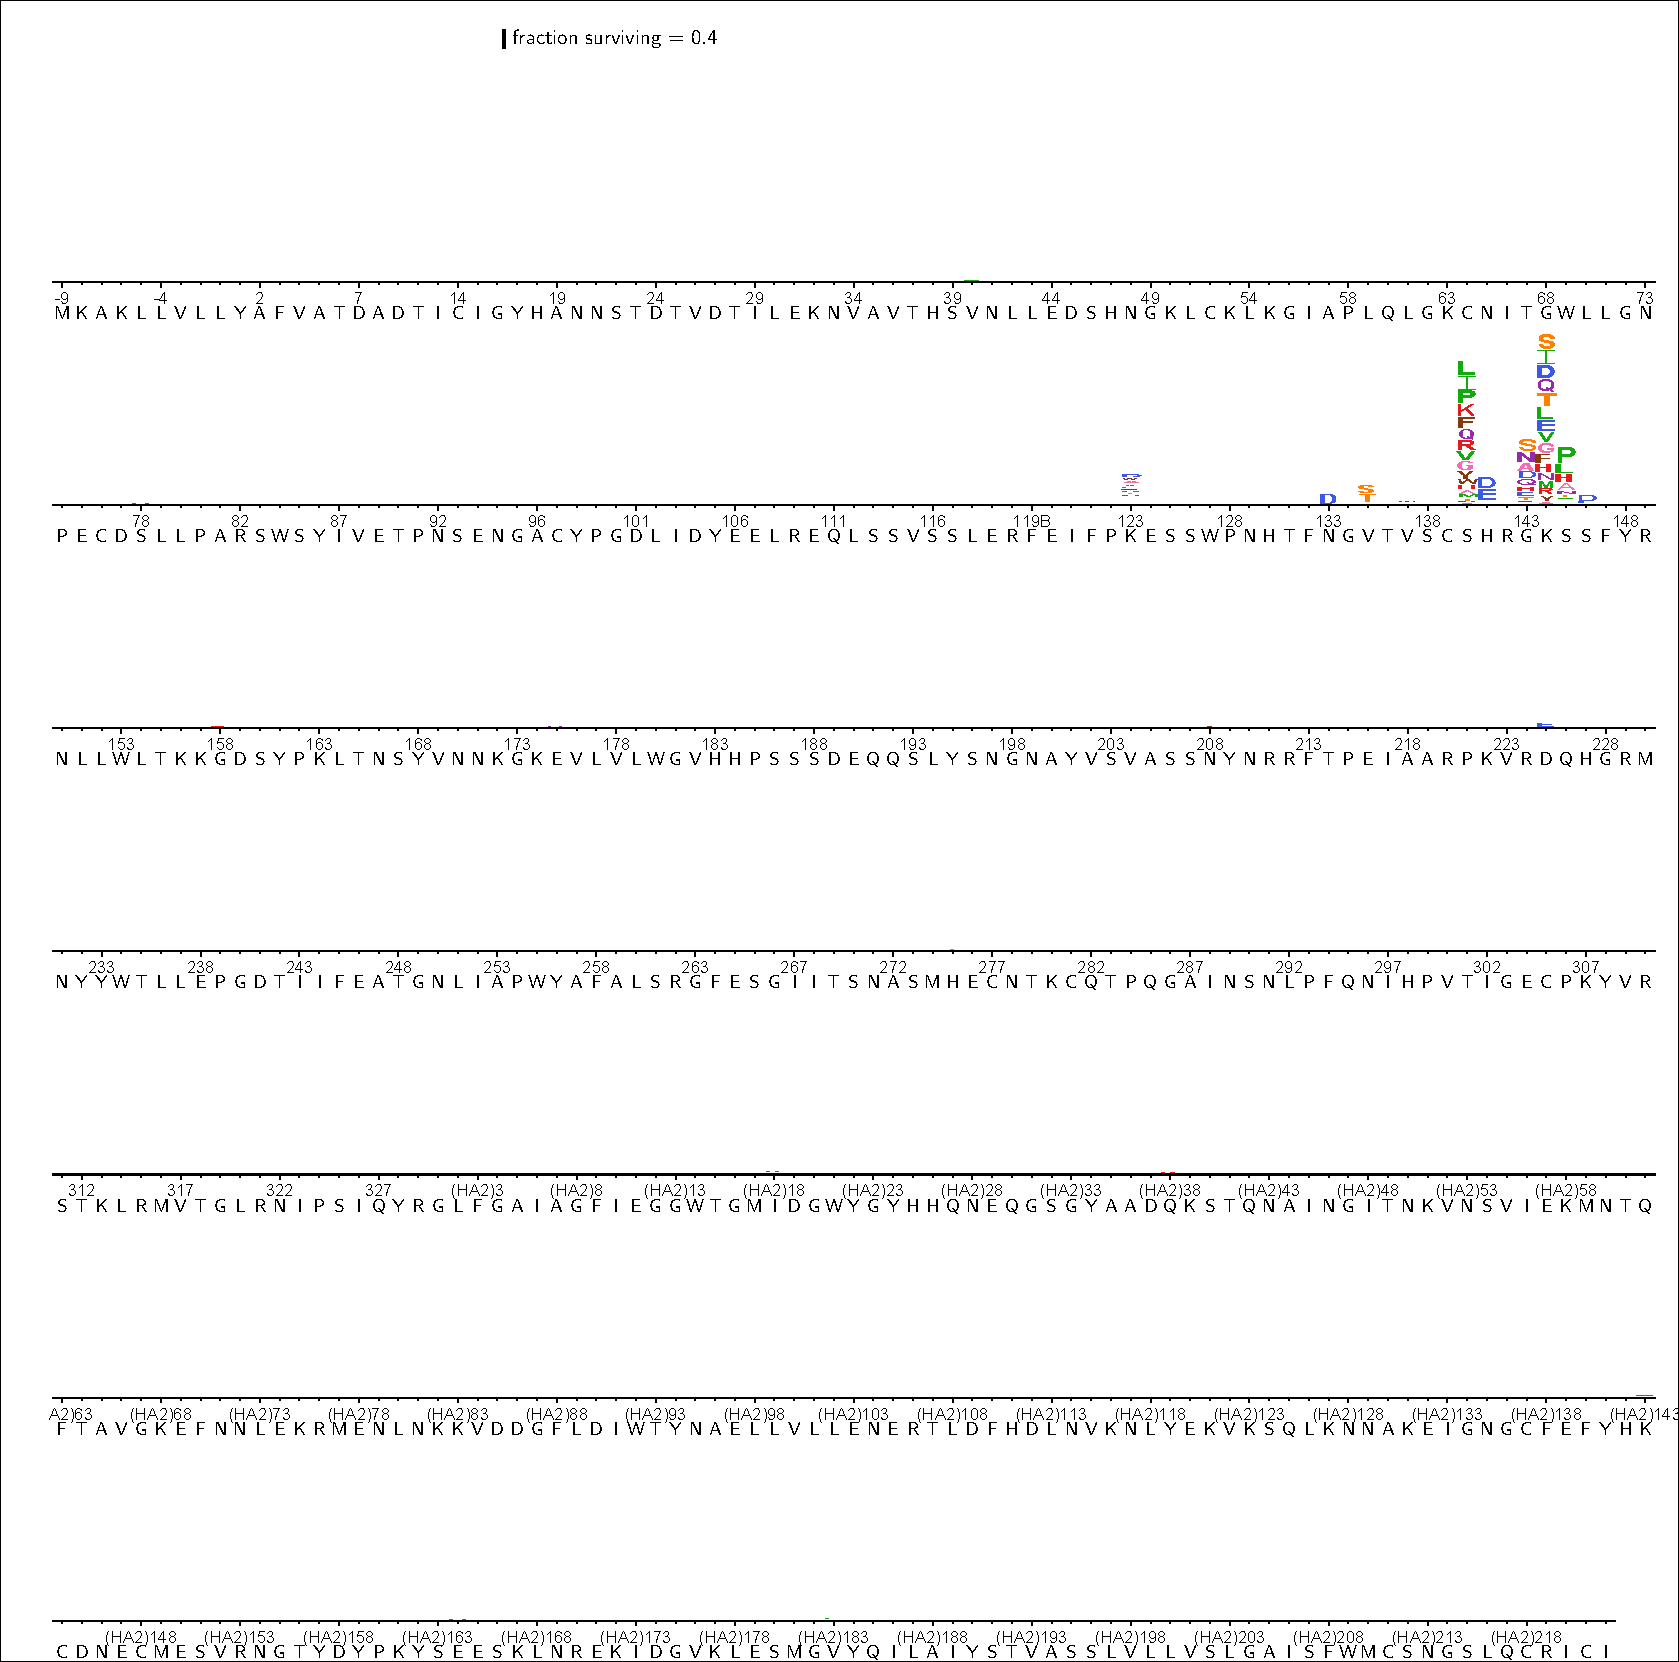
\includegraphics[trim=0.1cm 0.02cm 0.1cm 0.03cm,clip=true,width=\textwidth]{figs/logoplots/H17L19_fracsurvive.pdf}}
\caption{\label{suppfig:H17L19logo}
CAPTION}
\end{suppfigure}

\begin{suppfigure}
\centerline{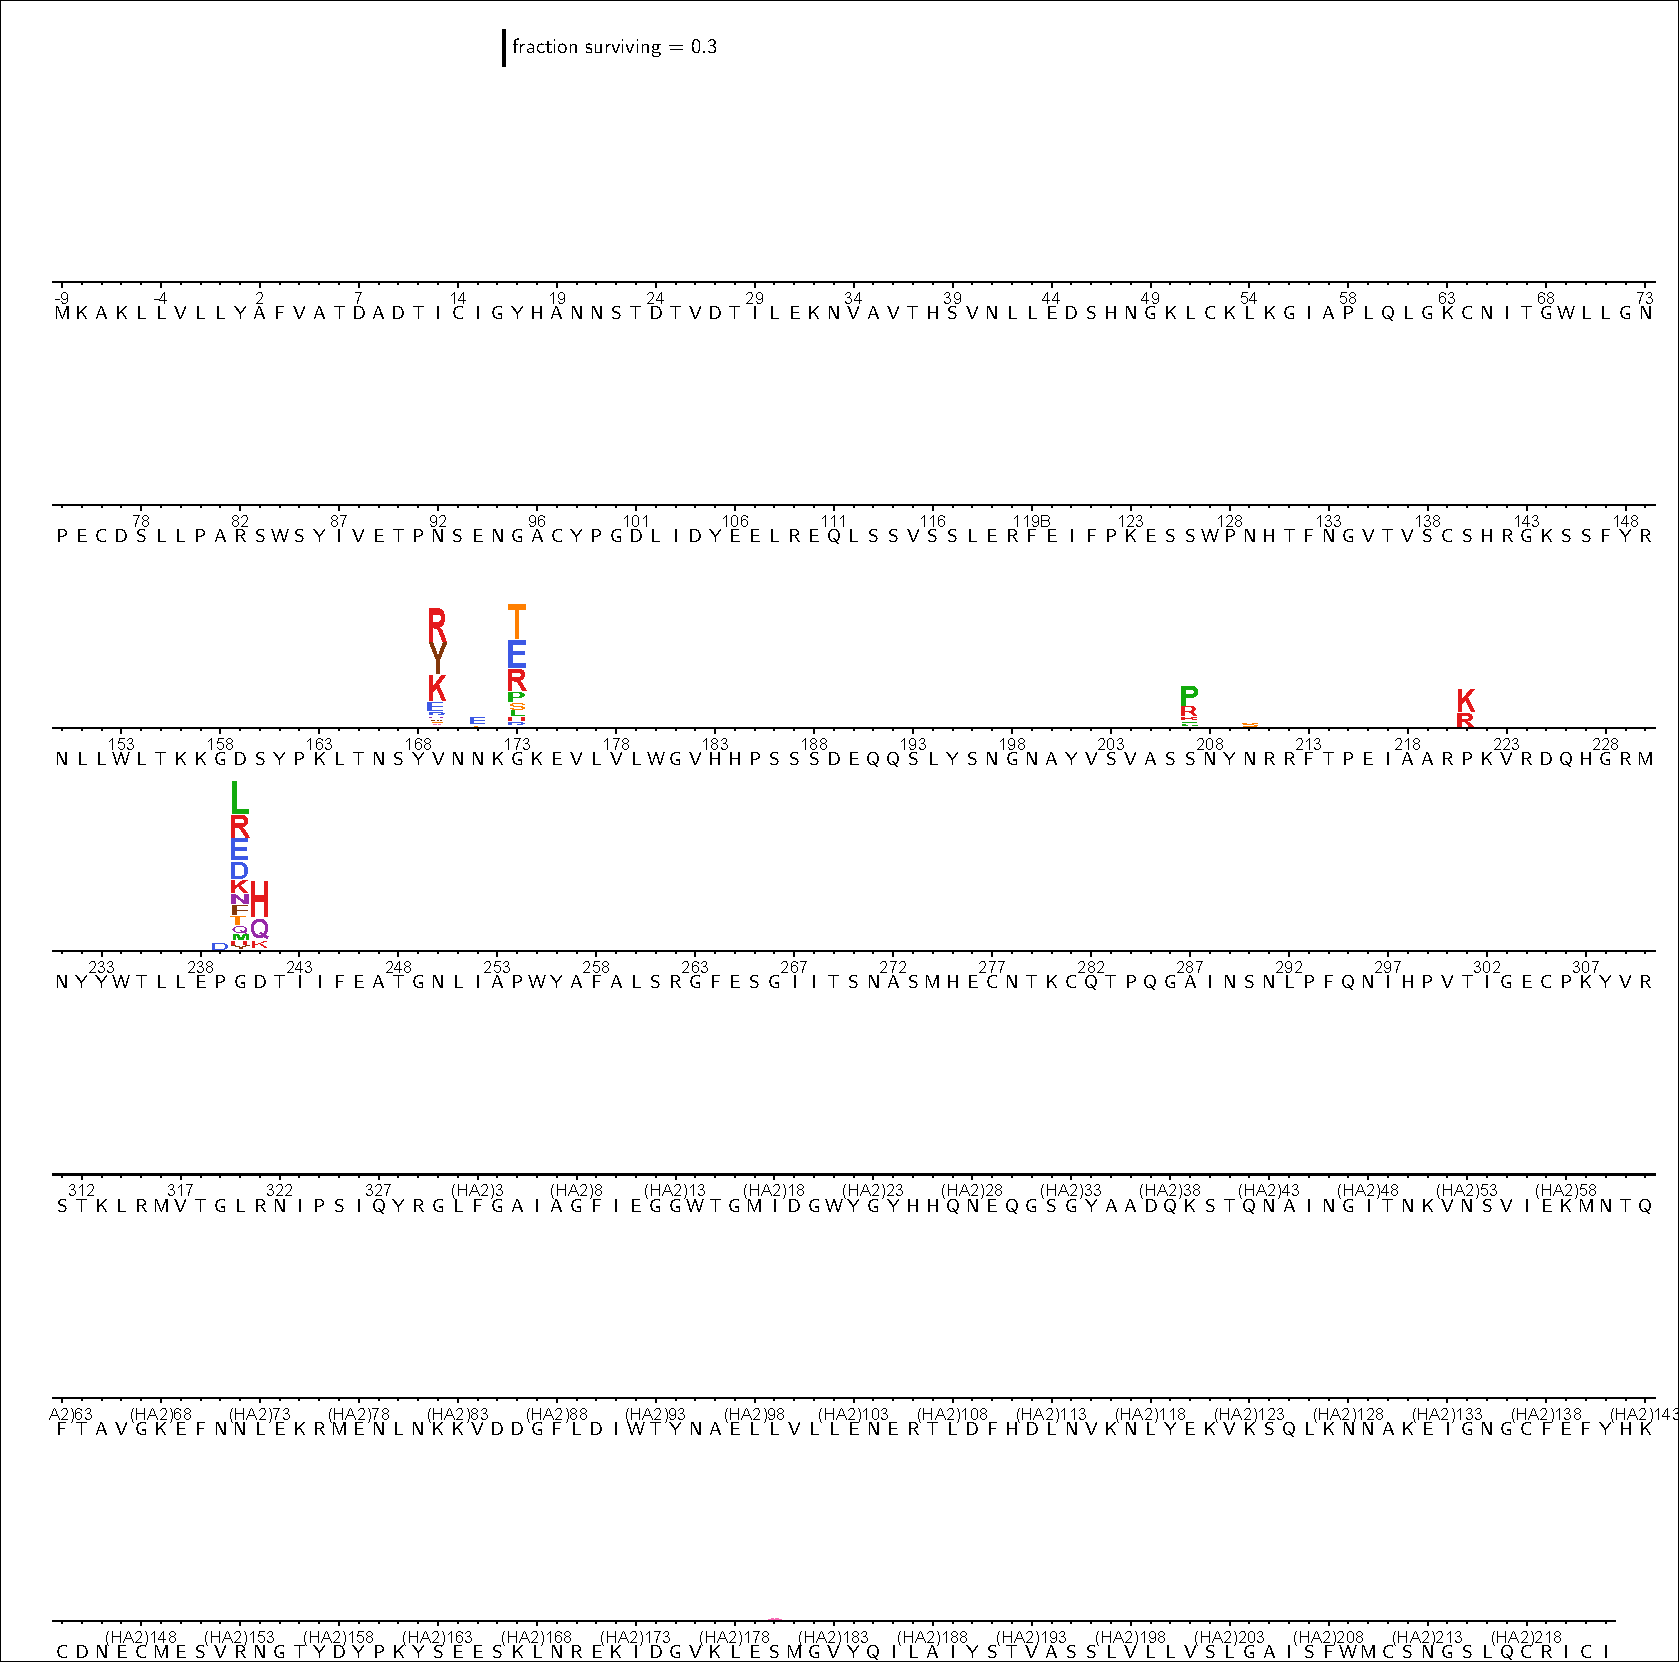
\includegraphics[trim=0.1cm 0.02cm 0.1cm 0.03cm,clip=true,width=\textwidth]{figs/logoplots/H17L10_fracsurvive.pdf}}
\caption{\label{suppfig:H17L10logo}
CAPTION}
\end{suppfigure}

\begin{suppfigure}
\centerline{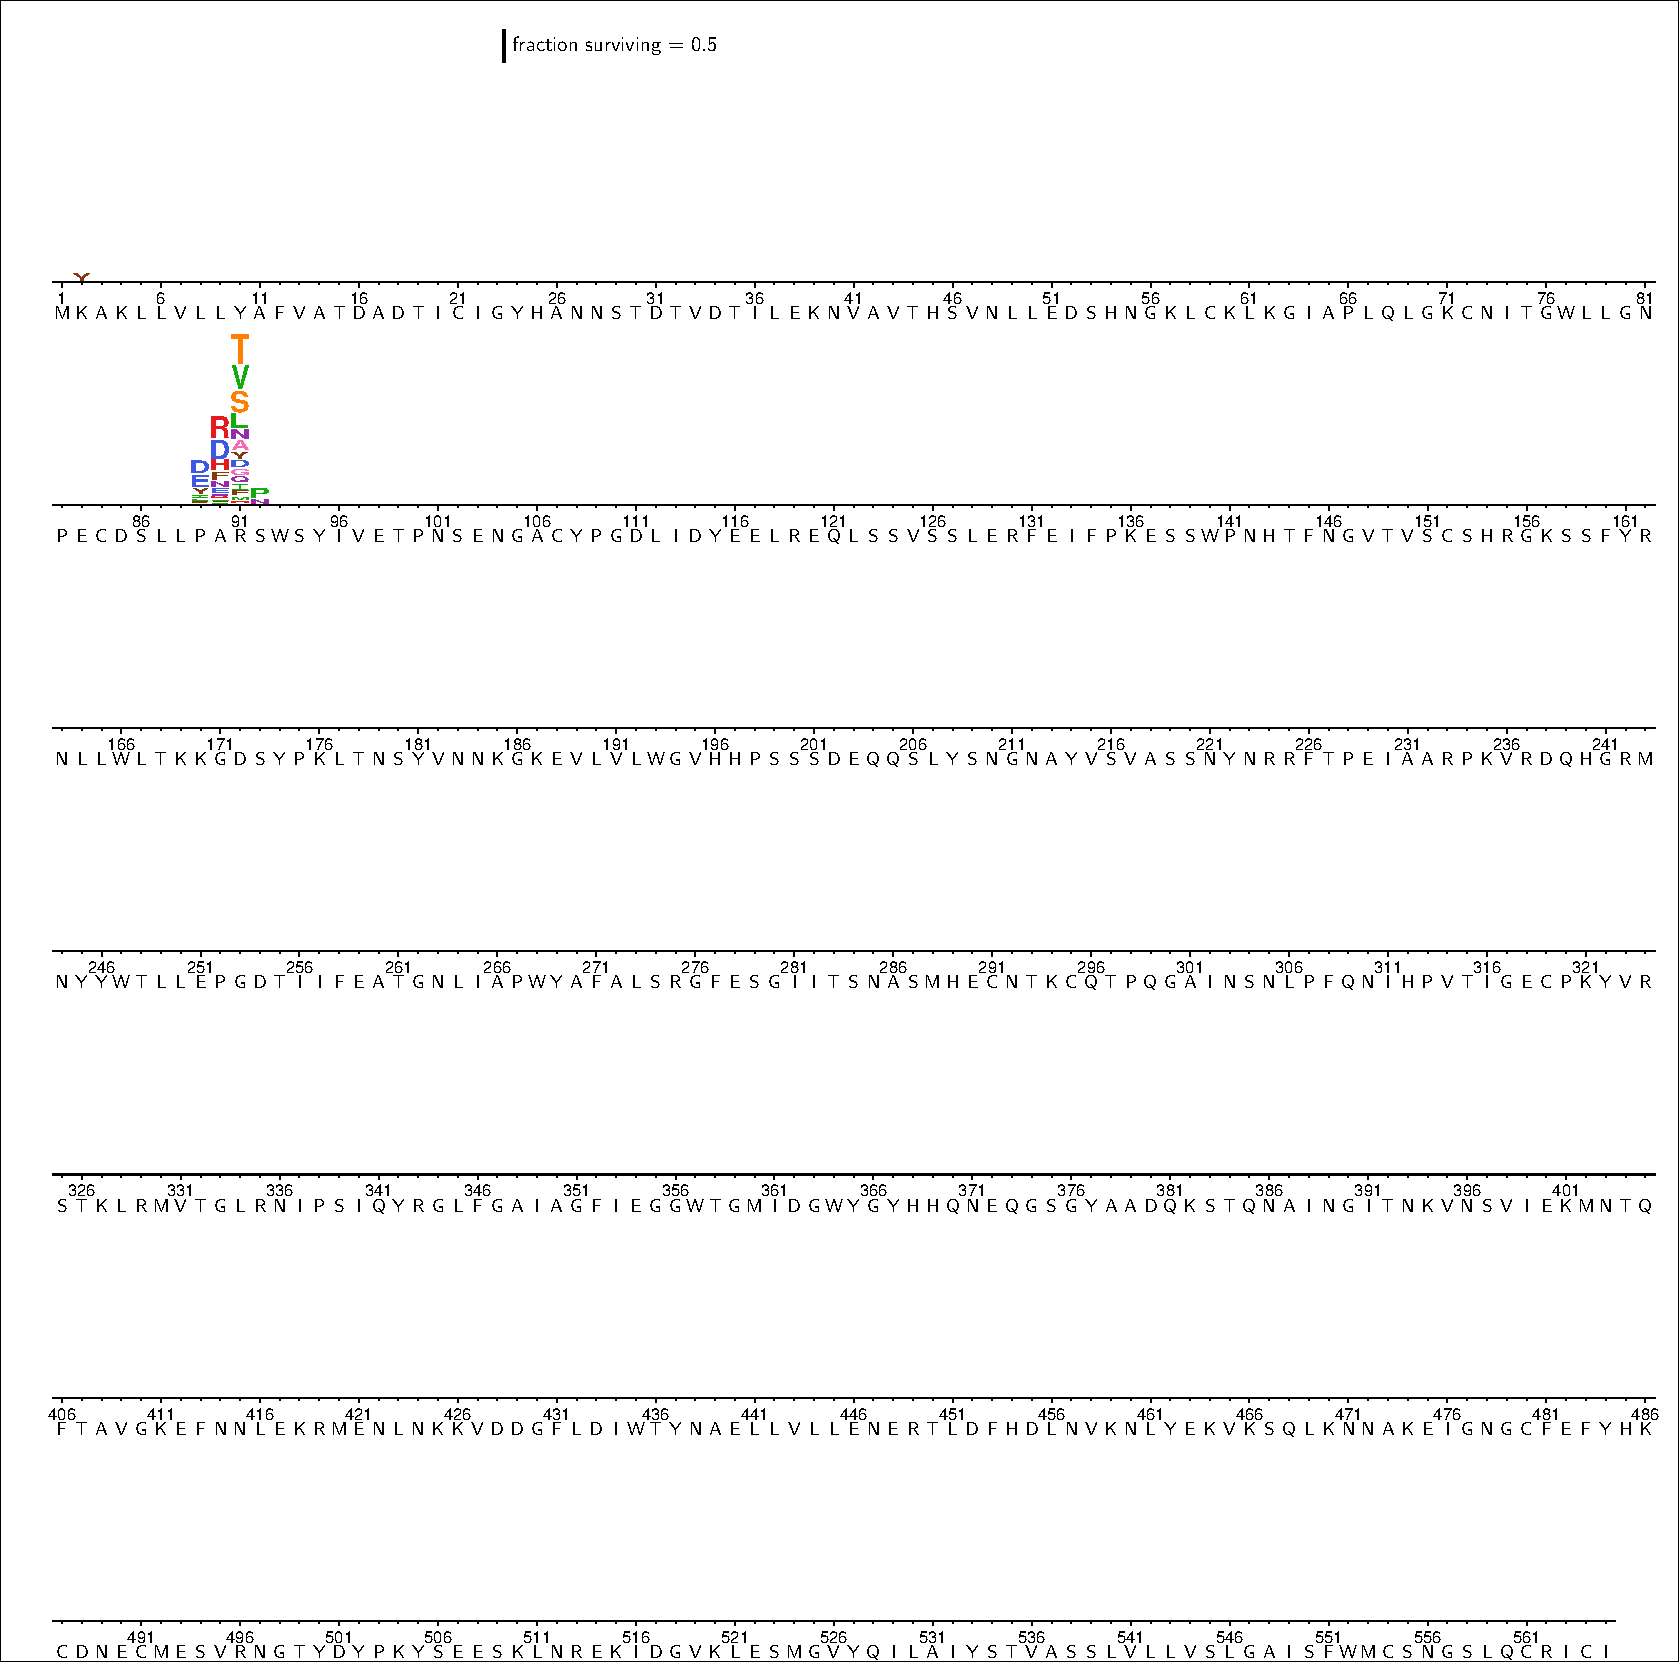
\includegraphics[trim=0.1cm 0.02cm 0.1cm 0.03cm,clip=true,width=\textwidth]{figs/logoplots/H17L7_fracsurvive.pdf}}
\caption{\label{suppfig:H17L7logo}
CAPTION}
\end{suppfigure}

\end{document}
